\documentclass{beamer}

% packages
\usepackage[slovak]{babel}
\usepackage[utf8]{inputenc}
\usepackage[T1]{fontenc}

% theme
\usetheme{metropolis}
\setbeamertemplate{footline}[frame number]

% title
\title{Lúštenie historických šifier na GRIDe}
\author{Bc. Martin Eliáš}
\date{Ing. Eugen Antal}
\institute{Slovenská technická univerzita v Bratislave}

\begin{document}
\maketitle

\begin{frame}{Motivácia}
	\begin{itemize}
    \item Grid vrámci STU
		\item Zjednodušenie práce pre výskumníkov
		\item Využitie dostupných prostriedkov
    \item Ušetrenie času a peňazí
  	\end{itemize}
\end{frame}

\begin{frame}{IBM iDataPlex}
  \begin{itemize}
      \item 52 výpočtových uzlov
      \item 624 CPU
      \item 2,5TB RAM
      \item 115TB HDD
      \item 6 TFlop/s (vs 93k Sunway TaihuLigth)
    \end{itemize}

  \begin{figure}
    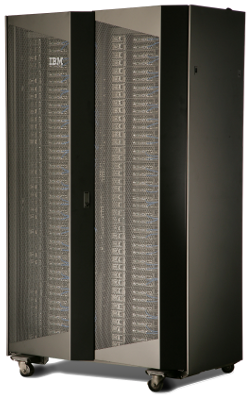
\includegraphics[scale=0.8]{img/hpc.png}
  \end{figure}
\end{frame}

\begin{frame}{Práca za zimný semester}
	\begin{itemize}
      \item Zoznámenie sa s gridom
		  \item Štúdium paralelných problémov
      \item Technológie
  		\item Prvé experimenty s bruteforce útokom
  	\end{itemize}
\end{frame}

\begin{frame}{Paralelizmus}
  \begin{itemize}
      \item Definícia
      \item Synchronizácia
      \item Komunikácia
      \item Návrh
    \end{itemize}
\end{frame}

\begin{frame}{Framework}
  \begin{itemize}
      \item OpenMPI a C++
      \item Skript na generovanie projektov a ich spúštanie
      \item Stavebné bloky (Runner, Communicator, ...)
    \end{itemize}
\end{frame}

\begin{frame}{Plán na letný semester}
	\begin{itemize}
  		\item Dokončenie frameworku
  		\item Slovníkový útok
  		\item Experiment s PGA
  	\end{itemize}
\end{frame}

\section{Ďakujem za pozornosť}

\end{document}
\grid
